
\pagestyle{fancy}
\chapter*{Introducci\'on}
\addcontentsline{toc}{chapter}{Introducci\'on}
%\mark{Introducci\'on}

\section*{El Sol}
\addcontentsline{toc}{section}{El Sol}

\vspace{0.2 cm}
{\renewcommand{\baselinestretch}{1.5}
{\footnotesize
\begin{flushright}
\begin{minipage}[h]{6cm}
\raggedleft{{\it solo es una bola de gas incandescente\\... cierto?}}
\end{minipage}
\end{flushright}}
\vspace{0.5cm}

\selectlanguage{spanish}

\noindent El Sol es la estrella m\'as cercana a nosotros (la siguiente est\'a unas 268 000 veces m\'as lejos) y por lo tanto es el objeto astron\'omico que con mayor intensidad influye en nuestro  vivir  cotidiano y en la curiosidad humana. Cuando se escudri\~na en el registro hist\'orico de las  civilizaciones antiguas se encuentra que, desde \'epocas remotas, el Sol ha tomado un papel de  importancia relevante en las visiones cosmol\'ogicas y cosmog\'onicas de distintas sociedades para el entendimiento del mundo \citep[]{vazquez2006}.\\

Aunque la naturaleza de nuestra estrella hu\'esped  y su relaci\'on con el sostenimiento de la vida en nuestro planeta ha inquietado al hombre durante varias generaciones, solo hasta comienzos del siglo XVII fue cuando se inici\'o un estudio riguroso y sistem\'atico del mismo. Este nacimiento de la f\'isica solar, por decirlo de alguna manera, fue desencadenado en gran medida gracias a las observaciones de manchas oscuras en el Sol (hoy d\'ia conocidas como {\it manchas solares}�); por parte de {\it Johannes Fabricius}, {\it Cristoph Schreiner} y {\it Galileo Galilei} de forma independiente; que rompieron con la concepci\'on equivocada de un Sol apol\'ineo e inalterable y que dieron pie al nacimiento de una ciencia que se encargara de estudiar su din\'amica.\\

El Sol es el objeto central de nuestro sistema solar y contiene un $99.8\%$ de la masa total del sistema. El Sol en s\'i mismo es una estrella que orbita el centro de nuestra galaxia, la {\it V\'ia L\'actea}, con una velocidad de unos $217\, \text{km/s}$ y un periodo de revoluci\'on de unos 230 millones de a\~nos (la \'ultima vez que el Sol estuvo en esta parte de la galaxia fue cuando aparecieron los dinosaurios). Comparado con la poblaci\'on de estrellas en nuestra galaxia, el Sol es una estrella com\'un que tiene un tama\~no medio y se encuentra en la mitad de su vida activa. En lenguaje astrof\'isico, es una estrella de tipo espectral G2 y de clase V en luminosidad, localizada en la secuencia principal del diagrama Hertzprung-Russell. De acuerdo con los modelos, el Sol ha permanecido en la secuencia principal por cerca de unos 5 000 millones de a\~nos y le restan otros 5 000 millones de a\~nos antes de que pase a la fase de las gigantes.\\

Uno de los encantos que tiene el estudiar el Sol hoy en d\'ia es que es aquella estrella de la que obtenemos la mayor cantidad de energ\'ia, suficiente como para estudiar su espectro en gran detalle y manejar una cadencia temporal muy peque\~na. Con m\'etodos indirectos es posible generar im\'agenes de la estructura superficial de otras estrellas cercanas. Pero con el Sol la historia es diferente; usando telescopios y t\'ecnicas comunes de la astronom\'ia es posible resolver estructuras por debajo de los 700 km de tama\~no  en su superficie, que representa la resoluci\'on espacial l\'imite con la que se trabaja en la presente tesis. Por su extrema cercan\'ia, tambi\'en es comparativamente sencillo estudiar la estructura de su atm\'osfera y los efectos de origen magn\'etico que tienen lugar all\'i, como es el caso de las fulguraciones solares (fen\'omeno de mayor inter\'es en este trabajo), las eyecciones coronales de masa, las manchas solares, las f\'aculas, los agujeros coronales, las esp\'iculas, {\it plages}, entre otros.\\

\renewcommand{\baselinestretch}{1.0}

\begin{wrapfigure}[15]{r}{0.41\textwidth}
\begin{center}

\includegraphics[width=0.32\textwidth]{Sun_in_hands.png}
\caption{El tama\~no aparente del Sol sobre nuestro cielo es de unos $\sim 32$ minutos de arco, un poco m\'as grande que medio grado.}
\label{solar-size}
\end{center}
\end{wrapfigure}

El Sol es el objeto m\'as brillante en nuestro cielo; es 12 magnitudes m\'as brillante que el segundo objeto m\'as brillante de una noche despejada y clara, la Luna llena. Su radiaci\'on es la responsable del calentamiento lum\'inico de la superficie terrestre, y por tanto un factor determinante del clima y en la sostenibilidad de la vida. El viento solar es quien nos separa del medio interestelar impidiendo que una gran cantidad de part\'iculas penetren nuestro sistema solar y puedan generarnos alg\'un da\~no. El campo magn\'etico solar nos protege de la incidencia de rayos c\'osmicos muy energ\'eticos, pero a su vez eventos muy violentos de origen magn\'etico que tengan lugar en su superficie podr\'ian alterar considerablemente nuestros sistemas de comunicaciones en tierra.\\

El Sol posee una estructura compleja. Esencialmente, este puede ser descrito como un conglomerado gigante de Hidr\'ogeno y Helio con un peque\~no porcentaje de elementos pesados aproximadamente en una relaci\'on de masa en su superficie de $\sim73.46\%$, $\sim24.85\%$ y $\sim1.69\%$ en masa, respectivamente. Debido a su gran masa la auto-gravitaci\'on mantiene a la estructura en forma de esfera casi completamente perfecta. El peso de las capas exteriores de gas incrementan la presi\'on en las regiones internas del Sol y dan lugar a los fen\'omensos de fusi\'on termonuclear que mantienen a la estrella en un constante equilibrio hidrost\'atico.


\subsection*{Estructura Interna}
\addcontentsline{toc}{section}{Estructura Interna}

 En el n\'ucleo solar la densidad, la presi\'on y la temperatura son tan altas del orden de 150 g/cm$^3$, $2.5\times 10^{17}$ din/cm$^3$ y 13 millones de kelvin respectivamente, que forman el ambiente propicio para que tengan lugar reacciones de fusi\'on termonuclear cuyo proceso principal es la quema de Hidr\'ogeno en Helio. Como resultado de este proceso, se tiene la producci\'on de energ\'ia en forma de radiaci\'on electromagn\'etica que involucra fotones de muy altas frecuencias y una alta emisi\'on de neutrinos. Debido a la alta densidad del medio, dichos fotones son continuamente absorbidos y re-emitidos por los iones cercanos, de manera que esa gran cantidad de energ\'ia producida en el interior es suave y lentamente radiada hacia el exterior de la estrella. Seg\'un esto, los fotones que hoy est\'an alcanzando la superficie de la tierra fueron generados en el interior solar apenas cuando el {\it Homo Sapiens} estaba apareciendo, o sea hace unos 170 000 a\~nos \citep[]{mitalas1992}.\\

\begin{SCfigure}
\centering
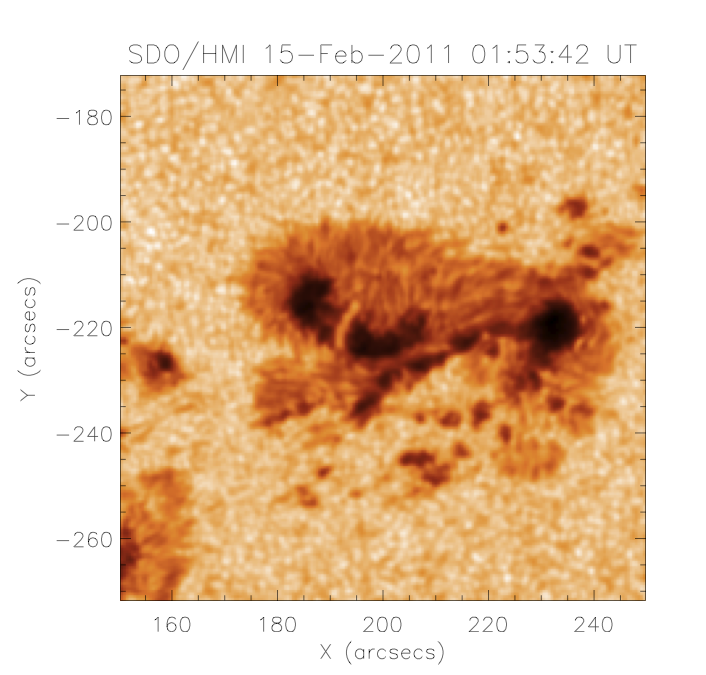
\includegraphics[width=0.63\textwidth]{resolution.png}
\caption{Regi\'on activa SOL2011-02-15T01:52 X2.2 registrada por SDO/HMI. Imagen de la ``superficie'' solar (fotosfera) con una resoluci\'on de $\sim 100$ km. Los gr\'anulos se ven en todas partes como peque\~nas zonas claras rodeadas por regiones oscuras. Sus formas se deben a que conforman la parte alta de la zona convectiva donde la energ\'ia se transporta desde el interior v\'ia el movimiento del gas. En la superficie el gas se enfria debido a que la energ\'ia se radia hacia el exterior. Las l\'ineas de campo magn\'etico fuertemente localizadas son las responsables de generar las zonas oscuras que se ven (manchas solares) como consecuencia de un decremento en la eficiencia del transporte radiativo en dicho lugar.}
\label{solar-size}
\end{SCfigure}

Aproximadamente a 0.7 radios solares del centro el mecanismo de transporte energ\'etico por {\it radiaci\'on} deja de ser eficiente. En ese lugar el gas se calienta, se expande, se vuelve din\'amico y se eleva hasta la superficie solar creando lo que se conoce como {\it celdas convectivas} que se encargan de transportar el gas caliente hasta la superficie donde se enfr\'ian y caen nuevamente para ser calentados y repetir el proceso una vez m\'as. Este flujo de gas transporta la energ\'ia hacia la parte externa del Sol donde la temperatura se reduce a unos $\sim 5\,700$ K y la densidad es lo suficientemente baja como para que los fotones puedan escapar de all\'i relativamente f\'acil, es decir, sin demasiadas interacciones con el plasma circundante. La regi\'on externa de donde recibimos la mayor cantidad de fotones \'opticos es com\'unmente llamada la {\it superficie solar} o {\it fotosfera} (esfera de luz), aunque no sea una capa s\'olida propiamente dicha.\\

La mayor\'ia de los fotones que recibimos provienen de all\'i y se encuentran en la regi\'on visible del espectro electromagn\'etico. Esta es muy probablemente la raz\'on por la que los seres vivos, en sus procesos de evoluci\'on pasados, desarrollaron \'organos de visi\'on que son mayormente sensibles en esta parte del espectro. Hacia afuera de esta capa se extiende radialmente la atm\'osfera solar, con un decremento de la densidad. Esta transici\'on ocurre acompa\~nada de un aumento en la temperatura que a\'un no est\'a completamente entendido y que alcanza unos cuantos millones de Kelvin. Por lo tanto debe existir una capa que tenga una temperatura m\'inima. Los modelos est\'andar proponen que esta capa se encuentra a una altura promedio de 500 km sobre la fotosfera y suponen una temperatura muy cercana a los 4000 K, suficientemente baja como para permitir la formaci\'on de mol\'eculas tales como el CO y/o el vapor de agua. A los dos lados de esta capa la temperatura se incrementa. Tambi\'en, en los modelos est\'andar, se considera que la capa posterior a esta se extiende unos 1 500 km hacia el exterior y alcanza temperaturas de los 8 000 a 10 000 K. Esta capa se conoce como la {\it cromosfera}. Enseguida a ella se encuentra la {\it regi\'on de transici\'on} donde la temperatura se incrementa abruptamente. Finalmente se tiene la parte m\'as externa de la atm\'osfera solar, llamada la {\it corona}, donde permanentemente se presenta un flujo continuo de part\'iculas que se mueve a lo largo de las l\'ineas de campo magn\'etico y conforma el {\it viento solar}. Dicho viento solar se extiende unas 100 000 veces el radio solar, mucho m\'as all\'a de \'orbita de Plut\'on, hasta la frontera de nuestro sistema solar, la {\it heliopausa}. Su interacci\'on con el medio interestelar crea un frente de choque, que est\'a siendo medido desde el 2009 por las sondas espaciales Voyager 1 y Voyager 2.\\

\renewcommand{\baselinestretch}{1.0}

\begin{wrapfigure}[29]{r}{0.58\textwidth}
\begin{center}
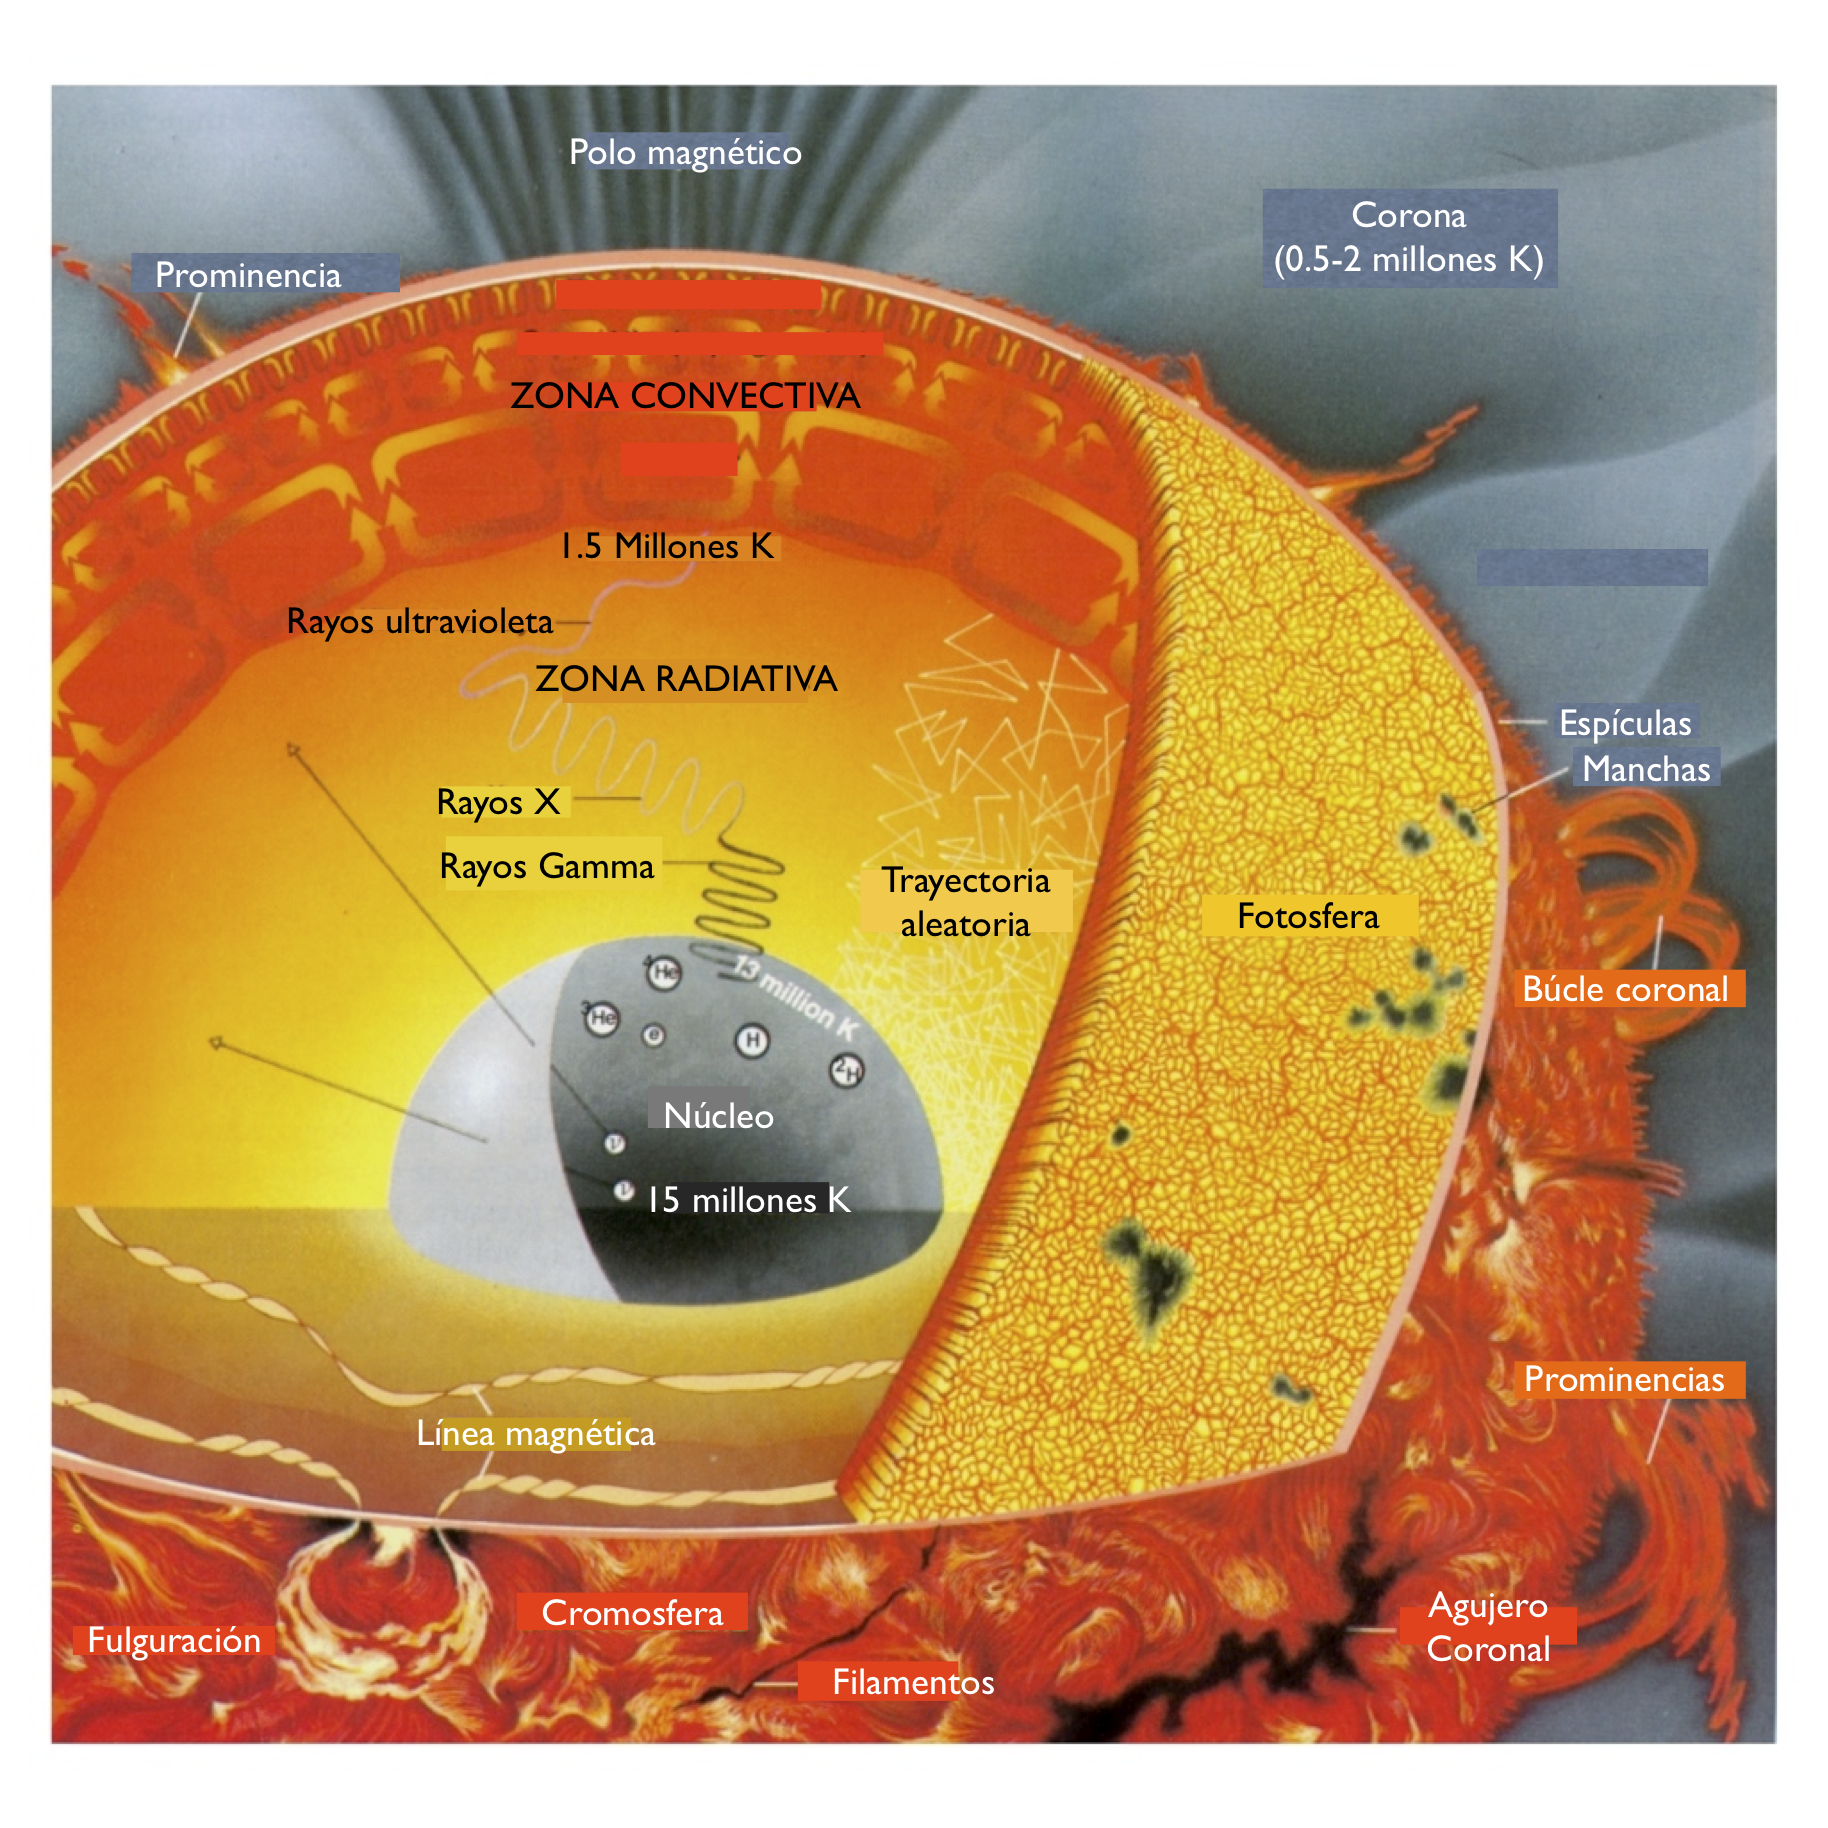
\includegraphics[width=0.58\textwidth]{sun.png}
\caption{Esquema de la estructura interna del Sol. Tres grandes zonas interiores en donde se genera y transporta la energ\'ia. Muchos fen\'omenos superficiales de origen magn\'etico.}
\label{sol}
\end{center}
\end{wrapfigure}

Detr\'as de esta estructura de capas, el Sol resulta ser a\'un m\'as complejo. Algunas otras propiedades que podemos describir brevemente, son:\\

- El Sol vibra. Considerado como una esfera auto-gravitante, compresible y en equilibrio, el Sol puede vibrar. Las perturbaciones en presi\'on y densidad generadas principalmente por las fluctuaciones convectivas se pueden propagar a lo largo de toda la estructura solar. Aquellas ondas con frecuencias cercanas entre s\'i pueden generar muchos modos normales de oscilaci\'on que sobre la superficie solar son vistas como patrones caracter\'isticos de diferentes configuraciones de interferencia constructiva. Estas vibraciones de baja amplitud (apenas unos cuantos cientos de metros por segundo en la fotosfera) pueden ser medidas y descompuestas en {\it modos propios} de oscilaci\'on mediante t\'ecnicas que involucran un an\'alisis por corrimiento Doppler y largos periodos de observaci\'on. La propagaci\'on de las ondas depende de las propiedades del medio. Es posible entonces suponer el camino contrario, mediante la medida de los patrones de vibraci\'on conocer algunas caracter\'isticas del medio propagador. Algunas ondas se propagan \'unicamente cerca de la superficie solar, pero otras, en cambio, pueden sumergirse completamente hasta el interior de la estructura. Estas \'ultimas ondas de las que se habla son la principal fuente de informaci\'on para inferir propiedades de estructura tales como la temperatura, densidad y presi\'on que puedan servir de {\it test} para evaluar la validez o no de un cierto modelo solar. De esto es justamente de lo que se encarga la {\it heliosismolog\'ia global} quien mediante los patrones de vibraci\'on determina diferentes valores de las propiedades globales de estructura. La {\it heliosismolog\'ia local} describe la din\'amica de los alrededores de una cierta perturbaci\'on que se da a nivel local, usualmente sobre la superficie del Sol (como es el caso de los fen\'omenos que se estudian en esta tesis).\\

- El Sol rota. La conservaci\'on del momentum angular de una nube de gas y polvo rotante puede dar pie al nacimiento de una estrella que despu\'es de contraerse rota a\'un m\'as r\'apido. Es ampliamente aceptado que el momentum angular de nuestra estrella fue removido durante sus primeras fases de vida por un fuerte campo magn\'etico anclado al medio interestelar circundante y por un viento fuerte. El remanente de dicho momentum angular inicial es el que vemos hoy en el Sol. El Sol no es un cuerpo r\'igido de manera que su periodo de rotaci\'on var\'ia con la latitud helioc\'entrica y con la distancia radial a su n\'ucleo. Hacia la zona equatorial el periodo sin\'odico de rotaci\'on en la superficie es de 27.2753 d\'ias, mientras que en los polos es de aproximadamente de 32 d\'ias. Mediante an\'alisis heliosismol\'ogicos se han encontrado registros de una rotaci\'on diferencial pero continua hasta una cierta profundidad (0.7 $R_\odot$), la {\it tacoclina}, a partir de la cual la rotaci\'on del Sol es como la de un cuerpo r\'igido que mantiene un periodo de rotaci\'on como el de las latitudes medias en la superficie. La rotaci\'on diferencial genera un flujo meridional de gas que va directamente a los polos cerca de la superficie y hacia el ecuador en la base de la zona convectiva.\\


\begin{figure}
\centering
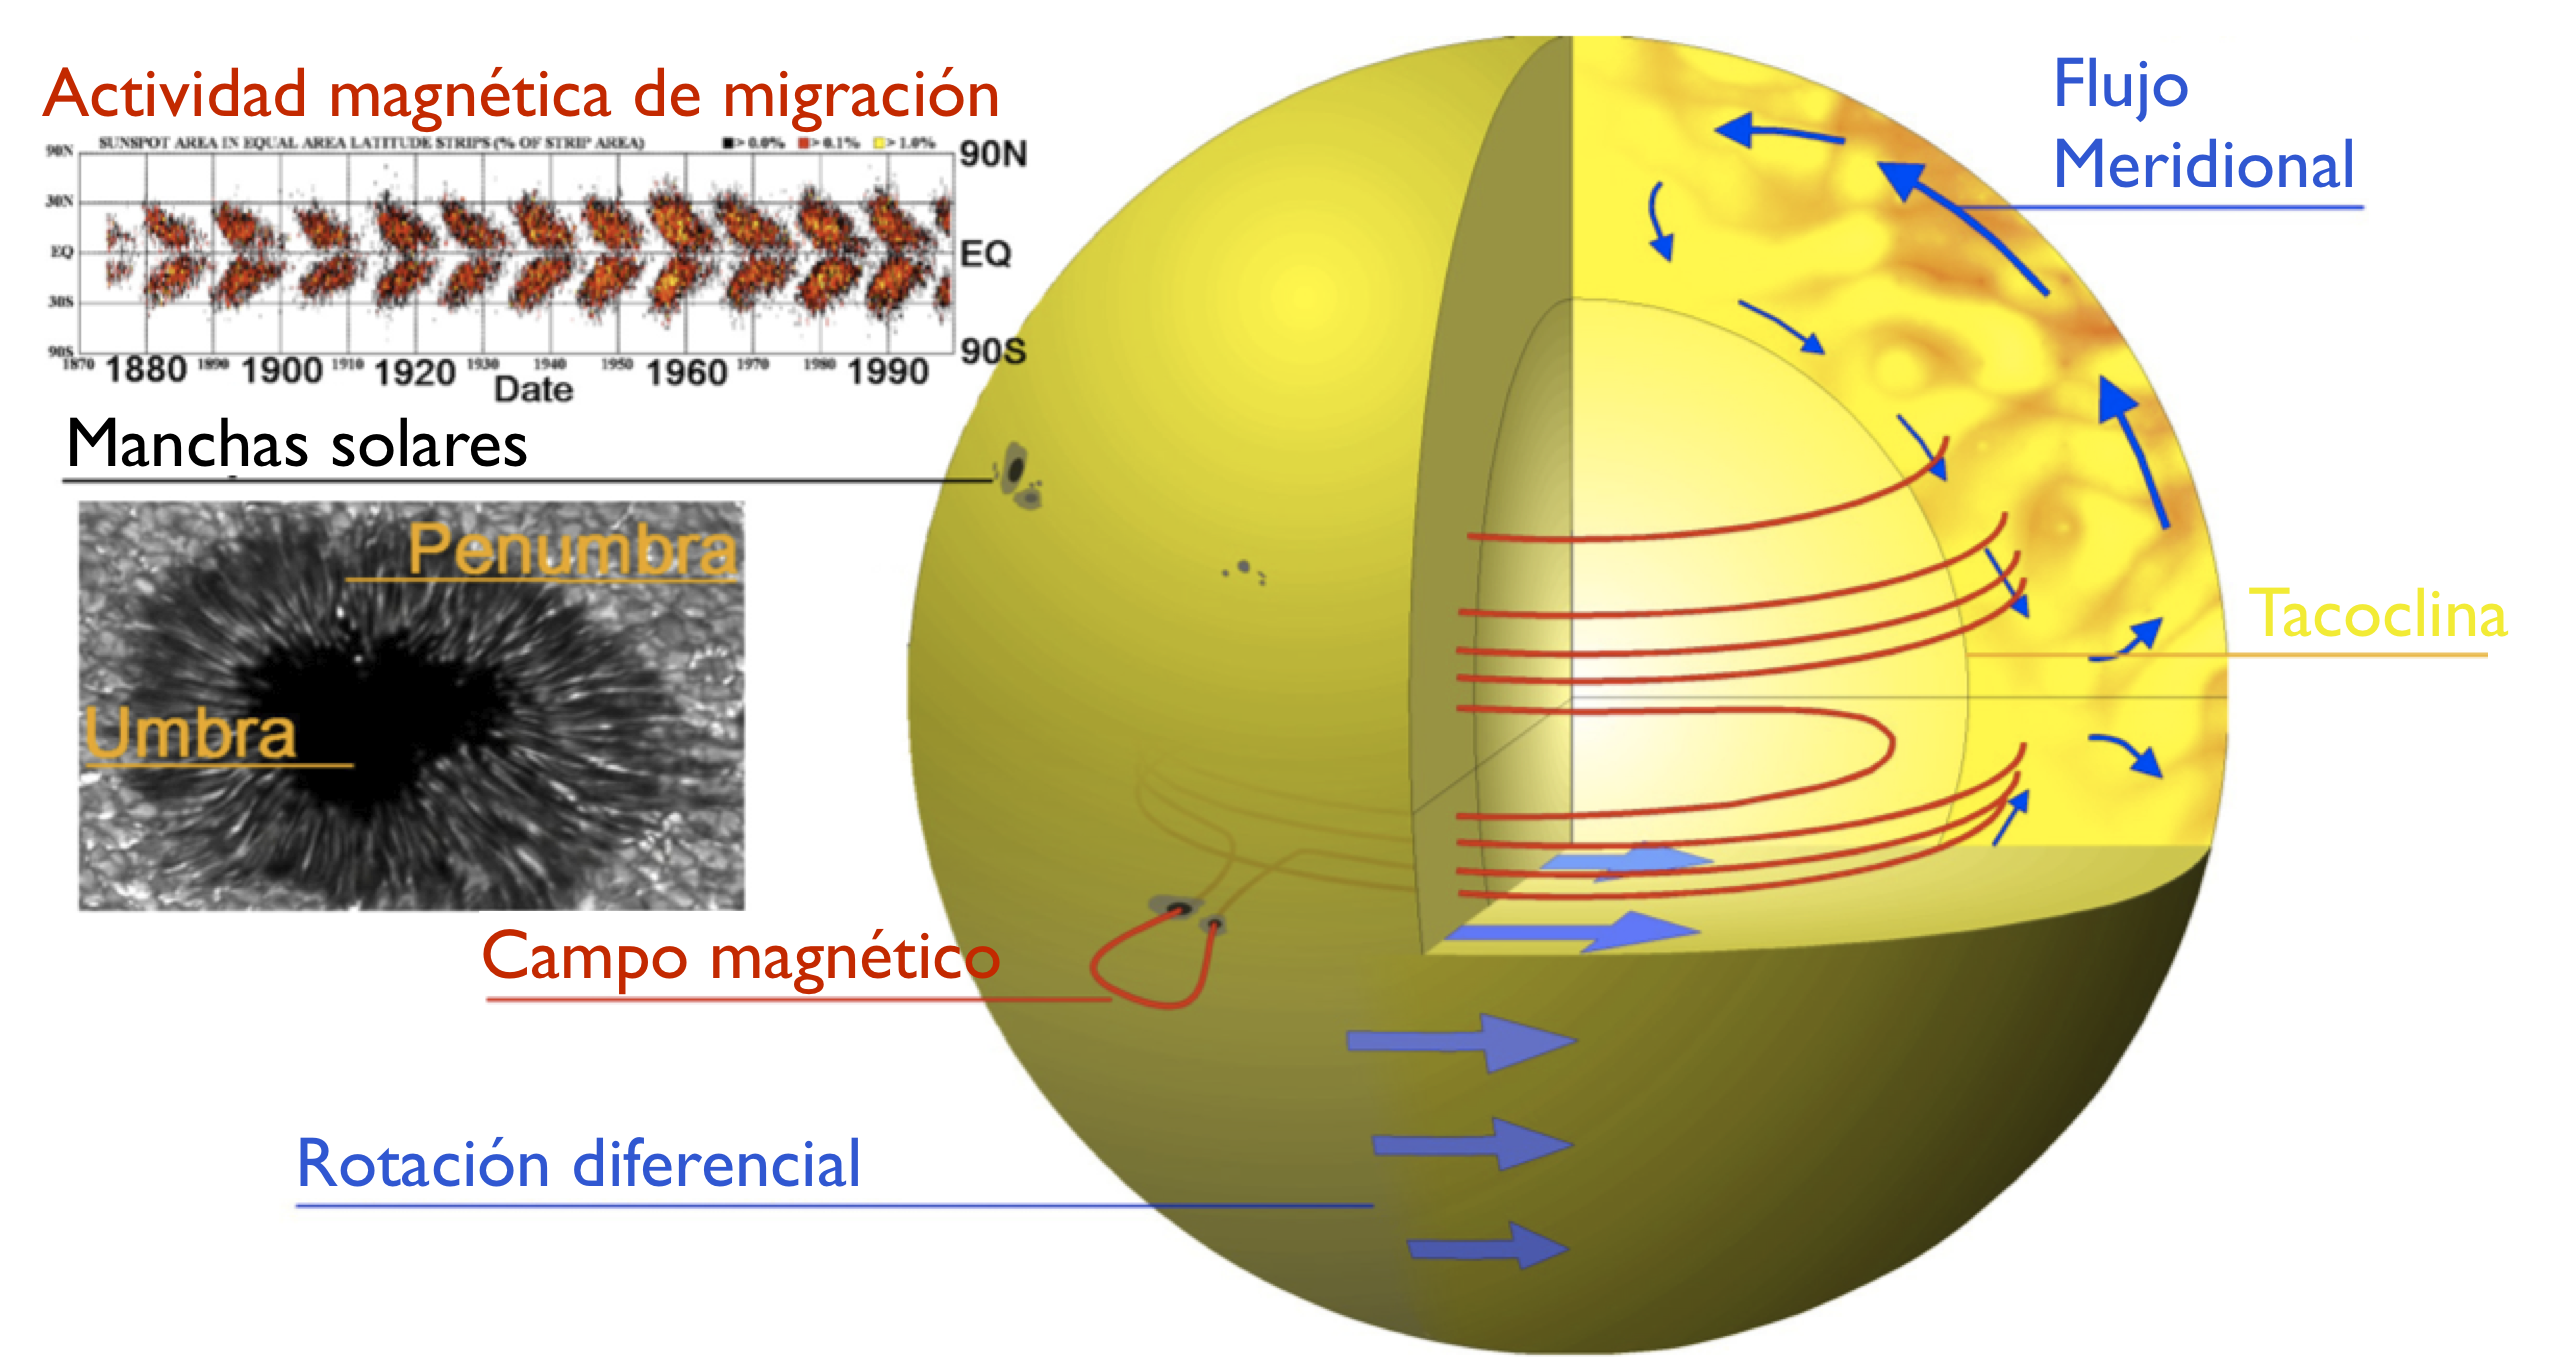
\includegraphics[width=1.0\textwidth]{sun_parts.png}
\caption{Representaci\'on gr\'afica de los diferentes aspectos del ciclo de actividad solar: Las l\'ineas de campo magn\'etico (rojas) se acumulan por la convecci\'on y la rotaci\'on diferencial (azul). El flujo meridional (azul), transporta la energ\'ia magn\'etica hacia el ecuador. En aquellas partes donde l\'ineas fuertes de campo magn\'etico penetren la fotosfera son generadas las manchas solares. Al inicio del ciclo solar las manchas aparecen en regiones de latitudes altas y a medida que transcurre el tiempo su aparici\'on se va desplazando hacia la zona ecuatorial. Referencia: Esta imagen fue tomada y modificada de \citep[]{kneer2003}}
\label{solar}
\end{figure}

- El Sol muestra una (compleja) actividad magn\'etica. El Sol posee una topolog\'ia de campo magn\'etico que macrosc\'opicamente mantiene una configuraci\'on dipolar d\'ebil. Sin embargo, la superficie solar puede albergar fen\'omenos que involucran muy fuertes y complicadas estructuras magn\'eticas observadas a trav\'es de su manifestaci\'on con las extra\~nas formas y din\'amicas que adopta el plasma superficial e.g. la baja eficiencia en el transporte energ\'etico que conduce a la aparici\'on de {\it manchas solares}. Toda la materia en el Sol se encuentra en forma de plasma debido a las temperaturas muy altas que se manejan all\'i. La alta conductividad que tienen las part\'iculas cargadas propias de un plasma hacen que despu\'es de que se ha alcanzado un cierto grado de equilibrio se genere un congelamiento de las l\'ineas de campo en \'el. La fuente de estas bien localizadas y fuertes l\'ineas de campo es a\'un hoy en d\'ia desconocido. Las teor\'ias de d\'inamo direccionan este problema sugiriendo que el campo magn\'etico dipolar d\'ebil es amplificado hacia la base de la zona convectiva por un movimiento estoc\'astico de la masa y retorcido producto de la convecci\'on y de la rotaci\'on diferencial.\\

- El Sol tiene ciclos. El Sol sufre fluctuaciones en el tiempo. Estos cambios se ven reflejados en la irradiancia total, en el viento solar y el campo magn\'etico. Esto sucede en un ciclo aproximadamente regular, como el ciclo de 11 a\~nos de las manchas solares, pero con aperidicidades en escalas extendidas de tiempo, como es el caso del m\'inimo de Mounder (un periodo de 75 a\~nos en el siglo XVII donde las manchas solares tuvieron un comportamiento extra\~no y que coincidi\'o con la llamada {\it peque\~na era de hielo}). Estas fluctuaciones modulan la estructura de la atm\'osfera solar, corona y viento solar, la irradiancia total, la aparici\'on de fulguraciones y eyecciones coronales de masa y tambi\'en indirectamente la incidencia en tierra o no de rayos c\'osmicos de fondo altamente energ\'eticos. Ninguna de estas variaciones ha sido completamente entendida y los efectos que desde el Sol se desprenden hacia la tierra a\'un son cuesti\'on de debate. La idea m\'as generalmente aceptada sobre los ciclos y fluctuaciones aperi\'odicas es que son causadas por cambios en la configuraci\'on del campo magn\'etico, frecuentemente entendidos y modelados mediante los mecanismos d\'inamo.\\

- El Sol evoluciona. Nuestra estrella se encuentra en este momento en la fase de la {\it secuencia principal}, donde la mayor fuente de energ\'ia es la fusi\'on nuclear de Hidr\'ogeno a Helio. Despu\'es de la fase inicial de acreci\'on de masa vino una fase entera de auto-gravitaci\'on en la que ha permanecido y permanecer\'a la mayor parte de su vida. En el caso del Sol, a\'un le restan otros cinco mil millones de a\~nos antes de que pase a un estado de evoluci\'on posterior que incluye una variaci\'on compleja en su radio y la quema de Helio como fuente de energ\'ia en su fase final de gigante roja. Al final de su vida, se cree que, terminar\'a como una {\it enana blanca}.\\

Dado que el tema que aqu\'i se plantea abordar involucra el entendimiento en m\'as detalle de las fulguraciones solares y de la heliosismolog\'ia local, son temas en los que se profundiza a continuaci\'on. Los lectores que est\'en interesados en encontrar m\'as informaci\'on general acerca del Sol pueden encontrarla en \citep[]{vaquero2009} y en las diferentes referencias que se citan all\'i.

\section*{Fulguraciones solares y otros eventos explosivos}
\addcontentsline{toc}{section}{Fulguraciones solares y otros eventos explosivos}

Una de las m\'as grandes diferencias entre los astrof\'isicos y los f\'isicos de otras \'areas es que los primeros no pueden reproducir ni analizar sus objetos de investigaci\'on en un laboratorio. Los astrof\'isicos dependen de lo que puedan obtener de sus observaciones. Part\'iculas que llegan de todas partes del universo son las mensajeras que traen informaci\'on de objetos muy distantes a nosotros. Naturalmente, muchas veces, esta informaci\'on puede ser muy dif\'icil de obtener o insuficiente. En este contexto los f\'isicos solares corren con una apreciable ventaja ya que su objeto de estudio es el m\'as cercano a nosotros en todo el universo. El Sol es la \'unica estrella de la que hoy es posible resolver espacialmente y en detalle su superficie mediante observaciones directas, permitiendo el estudio fino de estructuras cuya escala sea apenas de unos cuantos cientos de kil\'ometros. Adem\'as, es un objeto que est\'a siendo monitoreado permanentemente usando tanto estaciones en tierra como instrumentos espaciales que liberan miles de gigabytes al d\'ia. Aunque por razones evidentes no podamos variar los par\'ametros f\'isicos en este ``laboratorio'', s\'i podemos estudiar fen\'omenos extravagantes, que son imposibles de reproducir en tierra pero, que tienen lugar en todas partes del universo. Un ejemplo, que nos ata\~ne, de estos son las {\it fulguraciones solares}.\\

Entre los varios fen\'omenos que involucran una fuerte actividad magn\'etica en el Sol, las fulguraciones solares son particularmente fascinantes por la enorme potencia con la que se presentan. En una fulguraci\'on corriente se puede liberar una cantidad de energ\'ia del orden de $10^{32}$ erg ($10^{25}$ Joules) en unos cuantos segundos o minutos. Si por ejemplo se considera una fulguraci\'on cuya duraci\'on es de 10 minutos, su potencia puede ser estimada es unos $1.7\times10^{22}$ W que resulta ser unas 200 000 veces el consumo total de energ\'ia mundial durante el 2006 ($5\times10^{20}$ J) \citep[]{energy2006}. Se cree que dicha energ\'ia tiene un origen magn\'etico, y que es liberada cuando las l\'ineas de campo magn\'etico se reconectan en la corona. En estos procesos, las part\'iculas circundantes son aceleradas a altas energ\'ias y  liberadas hacia el espacio interplanetario a lo largo de las l\'ineas ``abiertas'' de campo o precipitadas hacia la cromosfera a trav\'es de las l\'ineas de campo del nuevo bucle reconectado. La interacci\'on colisional con el plasma de los alrededores produce una desaceleraci\'on o frenado completo del jet de part\'iculas emitiendo radiaci\'on bremsstrahlung (interacci\'on libre-libre) que puede ser observada en rayos-X (en este contexto tambi\'en llamados {\it footpoints}). El plasma cromosf\'erico se expande como producto del calentamiento producido por este tipo de interacciones, de manera que siendo menos denso sube a trav\'es de las l\'ineas de campo reconectadas estructurando la forma de bucle que vemos en rayos-X blandos o en EUV en este tipo de procesos. Esta din\'amica se conoce con el nombre de {\it evaporaci\'on cromosf\'erica}.\\

Los fen\'omenos m\'as explosivos de este tipo de eventos se observaron en la era moderna hacia finales de Octubre y comienzos de Noviembre de 2003. Para entonces, los sat\'elites con fines de telecomunicaci\'on geo-orbitantes tuvieron que apagarse temporalmente. Los astronautas en la {\it Estaci\'on Espacial Internacional} fueron forzados a permanecer en sus m\'odulos de servicio por un par de horas. Las aeronaves comerciales desviaron las rutas que pasaban por latitudes terrestres muy altas y en Suecia el suministro de corriente el\'ectrica colaps\'o dejando a cerca de 50 000 personas en oscuridad temporal. Estos eventos ayudan a mostrar la importancia que tiene la relaci\'on Sol-Tierra para la civilizaciones humanas modernas \citep[]{schwenn2006}.\\

Una fulguraci\'on en el Sol se define como un incremento espont\'aneo y r\'apido en la emisi\'on de radiaci\'on, en todo el rango del espectro electromagn\'etico (desde el radio hasta los rayos-$\gamma$), de alg\'un lugar bien localizado de la atm\'osfera solar. Este puede estar acompa\~nado de un calentamiento del plasma local, y un movimiento brusco de masa (por ejemplo una eyecci\'on coronal de masa). En fracci\'on de segundos una gran cantidad de la energ\'ia de la fulguraci\'on es transferida  a la aceleraci\'on de part\'iculas (principalmente, pero no exclusivamente, electrones). 

\begin{figure}
\centering
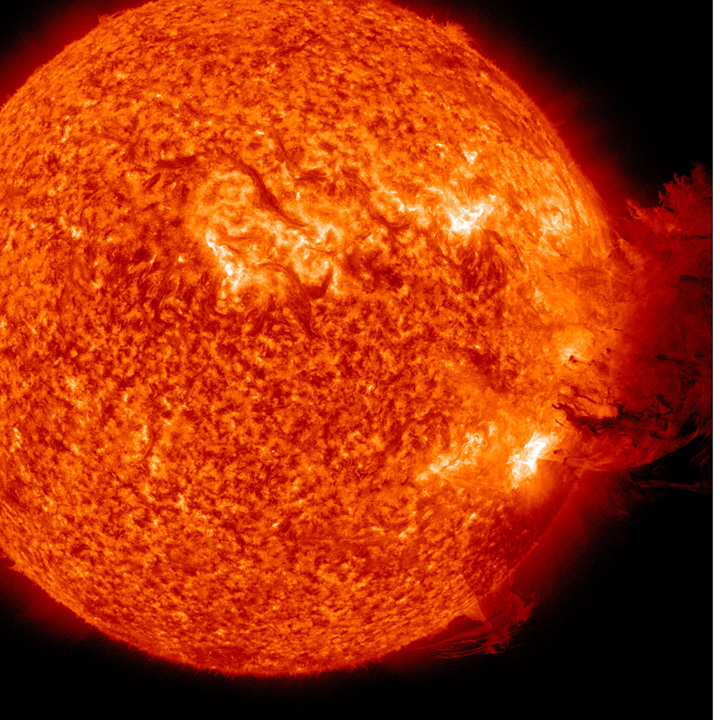
\includegraphics[width=0.99\textwidth]{sdoflare.jpg}
\caption{Fulguraci\'on tipo M2 (de tama\~no medio) junto con una eyecci\'on coronal de masa que ocurri\'o el pasado 7 de Junio de 2011 a las 01:41 TU. Tomada en EUV por SDO/AIA a 304\AA. La CME ten\'ia rumbo hacia la tierra con una velocidad de $\sim1 400$ km/s. Los efectos sobre la tierra fueron muy leves, apenas unas cuantas auroras. Imagen tomada de: sdo.gsfc.nasa.gov/gallery.}
\label{sdoflare}
\end{figure}

\subsection*{Fases de las fulguraciones solares}
\addcontentsline{toc}{subsection}{Fases de las fulguraciones solares}

Como se mencion\'o anteriormente, las fulguraciones solares emiten en un amplio rango del espectro electromagn\'etico. La intensidad de emisi\'on y la forma que toma la curva de luz para cada valor de frecuencia est\'an directamente asociadas a una variedad de diferentes procesos f\'isicos que se presentan seg\'un la din\'amica del fen\'omeno. Varios trabajos se han desarrollado en torno a la caracterizaci\'on de estos espetros y curvas de luz en busca de definir una especie de ``taxonom\'ia'' que permita distinguir las diferentes fases por las que tiene que pasar una fulguraci\'on \citep[]{mo2009,fletcher2011}.

\subsubsection*{Pre-fulguraci\'on}
\addcontentsline{toc}{subsubsection}{Pre-fulguraci\'on}

En esta fase la energ\'ia magn\'etica se acumula lentamente en la corona solar. Este proceso puede durar de entre unas cuantas horas a un par de d\'ias. Por medio de alg\'un mecanismo, que a\'un es tema de discusi\'on, la configuraci\'on de campo magn\'etico se desestabiliza y la energ\'ia es liberada espont\'aneamente. A esta antesala de la fulguraci\'on se le conoce tambi\'en como la {\it fase  precursora}. El aumento en la emisi\'on de radiaci\'on a diferentes frecuencias no necesariamente se presenta en el lugar de la explosi\'on, y depende de las propiedades f\'isicas que acompa\~nan al proceso. A partir de estas, se ha catalogado esta fase seg\'un las observaciones que se han obtenido. Estas clases son:\\

{\it - Fulguraciones hom\'ologas}. En algunas ocasiones las regiones activas presentan fulguraciones de baja intensidad y en movimiento que tienen lugar antes y muy cerca de la fulguraci\'on principal. Este fen\'omeno muestra que el campo magn\'etico, y en particular el torcimiento de las l\'ineas, tiene una din\'amica que lo hace cambiar en el tiempo. Tales cambios podr\'ian, eventualmente, generar el desencadenamiento de la gran explosi\'on.\\


{\it - Fulguraciones sympathetic}. Este tipo de eventos han sido observados en regiones magn\'eticas del Sol que se relacionan de manera cercana. Un ejemplo t\'ipico es la observaci\'on de fulguraciones casi completamente sincronizadas que ocurren en diferentes regiones del disco solar. Este fen\'omeno resulta ser muy llamativo ya que muestra fulguraciones ocurriendo en diferentes lugares que, en principio, podr\'ian ser transmitidas a otras zonas en donde eventualmente inducir\'ian fulguraciones mucho mayores.\\

{\it - Rayos-X blandos precursores}. Algunas veces es posible observar rayos-X blandos transitorios que pueden durar hasta unas cuantas decenas de minutos. En esta configuraci\'on, la distribuci\'on del campo magn\'etico en la corona es complicada y est\'a compuesta de muchos grandes y peque\~nos bucles. Algunas veces estos peque\~nos bucles interact\'uan con el bucle principal de la regi\'on activa. Esta interacci\'on, cuando se presenta, puede generar peque\~nas fulguraciones que pueden ser vistas en rayos-X blandos debido a la radiaci\'on t\'ermica que all\'i se presenta, pero quiz\'as lo m\'as importante de esta din\'amica es que esta interacci\'on puede llevar a contribuir a la desestabilizaci\'on del campo magn\'etico e inducir una fulguraci\'on a\'un m\'as grande.\\

{\it - Radiaci\'on precursora en radio}. Como se mencion\'o anteriormente, las fulguraciones solares radian en una amplia regi\'on del espectro electromagn\'etico. La radiaci\'on precursora en radio es un cambio en la intensidad y/o la polarizaci\'on de la radiaci\'on emitida en este rango del espectro por parte de la regi\'on activa observada sobre todo en microondas con una duraci\'on t\'ipica de las decenas de minutos.\\


{\it - Precursores en extremo ultra-violeta (EUV)}. Es el caso en el que se ve un acrecentamiento de la emis\'on en EUV en peque\~nos n\'ucleos localizados que despu\'es pueden ser correlacionados con la presencia de la fulguraci\'on. Tanto en este caso como en los precursores de radio las emisiones son asociadas con la reconfiguraci\'on de las l\'ineas de campo magn\'etico.\\


Frecuentemente estos {\it precursores} resultan ser indicadores directos o indirectos de la evoluci\'on del campo magn\'etico en regiones fulgurantes. Sin embargo, para estudiar los cambios reales del campo magn\'etico es necesario medirlo tanto en la corona sola como en la fotosfera. Varias t\'ecnicas son usadas con tal fin. Una de ellas hace uso de los magnetogramas vectoriales en busca de interpolar el campo magn\'etico en la corona y determinar su valor \citep[]{wheatland2000,wang2011}. En otras, se hace uso de las observaciones en radio de regiones {\it cuasi-transversales} donde es posible deducir el valor de campo magn\'etico en la corona \citep{Ryabov2005}. 

\subsubsection*{Fase impulsiva}
\addcontentsline{toc}{subsubsection}{Fase impulsiva}

Una de las formas m\'as sencillas de considerar una fulguraci\'on es la siguiente: Despu\'es de que la energ\'ia magn\'etica es almacenada durante la fase de la prefulguraci\'on se libera por alg\'un mecanismo de desestibilizaci\'on del campo magn\'etico coronal. Como resultado, el plasma local se calienta y las part\'iculas son r\'apidamente aceleradas. Los haces de part\'iculas no t\'ermicas se propagan a lo largo de las l\'ineas de campo magn\'etico alcanzando, eventualmente, la cromosfera y la fotosfera solar. As\'i como algunas de las part\'iculas aceleradas son precipitadas hacia la atm\'osfera solar, otras pueden salir en direcci\'on contraria (incluso como cantidades grandes de masa) hacia el espacio interplanetario.\\

\renewcommand{\baselinestretch}{1.0}

\begin{wrapfigure}[35]{r}{0.49\textwidth}
\begin{center}
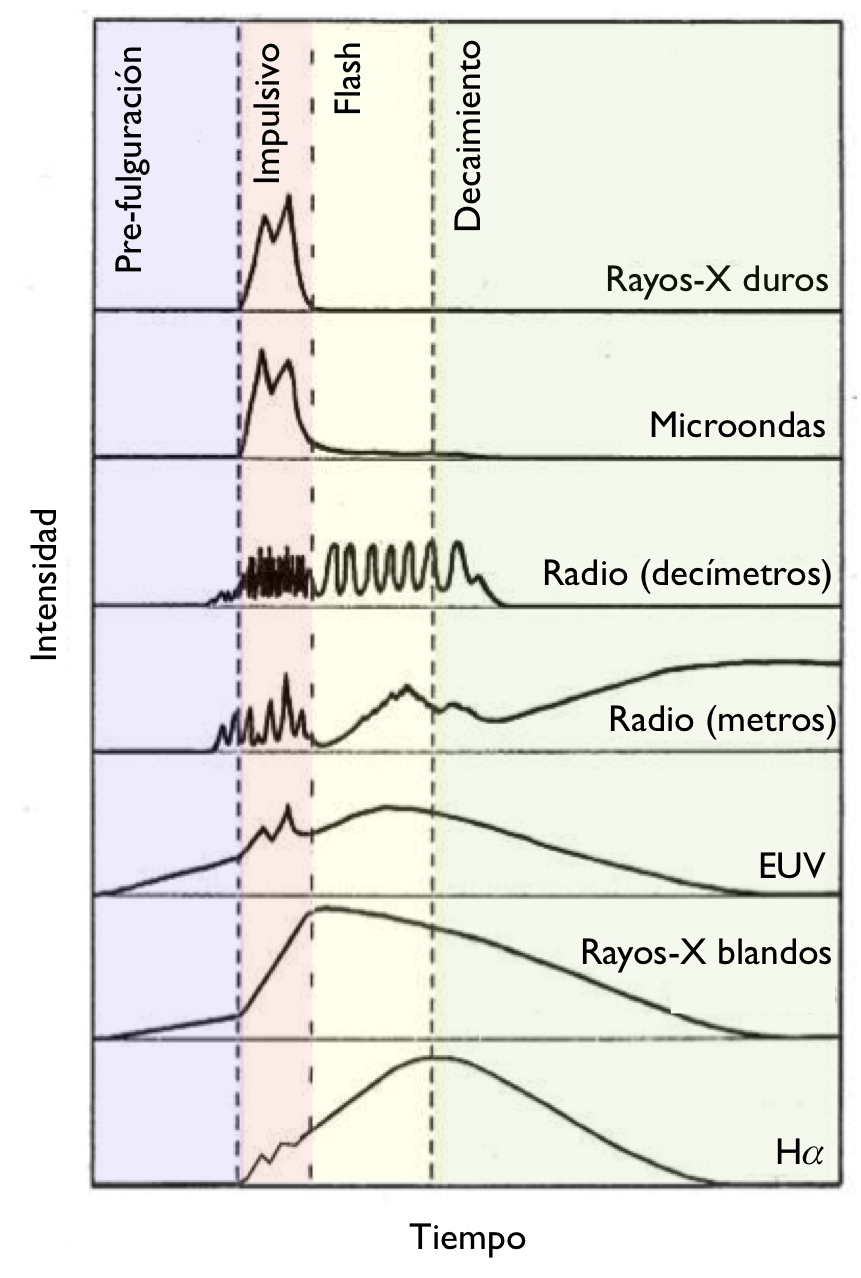
\includegraphics[width=0.49\textwidth]{lo.png}
\caption{Esquema general de los perfiles temporales de la emisi\'on en diferentes rangos del espectro electromagn\'etico de una fulguraci\'on solar. Figura tomada y adaptada de \citep[]{benz2002}.}
\label{sol}
\end{center}
\end{wrapfigure}

La fase impulsiva se caracteriza por un incremento r\'apido y brusco de la intensidad en todas las frecuencias. Varios estudios del perfil temporal del flujo en las fulguraciones solares han mostrado fluctuaciones que indican la presencia de un mecanismo impulsador que inyecta cierta cantidad de part\'iculas en el bucle \citep[]{aschwanden2004}. Durante esta fase es posible observar una gran variedad de tipos de radiaci\'on en diferentes lugares del arco magn\'etico. Estas emisiones, en particular en rayos-X y en radio, nos dan informaci\'on del mecanismo por el cual son aceleradas las part\'iculas y mediante el cual la liberaci\'on de energ\'ia tiene lugar durante esta fase impulsiva. Los rayos-X duros son producidos en la fotosfera en las bases del bucle (o los as\'i llamados {\it footpoints} en ingl\'es) v\'ia radiaci\'on de frenado, o {\it Bremsstrahlung}, por la colisi\'on del chorro de electrones con el ambiente cromosf\'erico denso (principalmente compuesto de iones). Cuando se habla de rayos-$\gamma$ casi siempre estos tienen un origen nuclear. As\'i, las l\'ineas observadas en este rango de frecuencias son debidas a la colisi\'on entre los protones acelerados en la fulguraci\'on y el plasma cromosf\'erico. La emisi\'on en {\it radio} es debida a otro mecanismo de radiaci\'on. Existen dos formas b\'asicas de producir un flujo neto en radio, por emisi\'on t\'ermica y no-t\'ermica. Este \'ultimo es debido a un efecto del movimiento de los electrones a lo largo de las l\'ineas de campo magn\'etico conocido como  radiaci\'on {\it giro-sincrotr\'on}. Se ha observado que el flujo en esta banda est\'a muy fuertemente correlacionado con la emisi\'on en rayos-X asociada a los {\it footpoints} en este tipo de eventos. Este hecho puede ser explicado si se supone que ambas poblaciones de electrones no-t\'ermicos, responsables de la emisi\'on en radio y en rayos-X duros, tienen un origen com\'un en la fulguraci\'on solar. La observaci\'on en {\it microondas} tiene una importancia bien particular, ya que se supone que esta emisi\'on se produce justo antes que las part\'iculas pierdan su energ\'ia v\'ia colisiones de forma que nos pueda brindar informaci\'on acerca del mecanismo por el cual fueron aceleradas dichas part\'iculas.

\subsubsection*{Fase del flash}
\addcontentsline{toc}{subsubsection}{Fase del flash}

En general todas las fulguraciones presentan un incremento en la intensidad sobre las l\'ineas de emisi\'on cromosf\'erica despu\'es de la fase impulsiva, particularmente en la l\'inea de H$\alpha$. Cuando el haz de part\'iculas aceleradas colisiona con el plasma cromosf\'erico, el calentamiento local genera l\'ineas de emisi\'on t\'ermica en el cont\'inuo de {\it Balmer}. De manera que, en una fulguraci\'on no solamente se producen rayos-X sino tambi\'en se emiten fotones en H$\alpha$. El t\'ermino {\it fase de flash} fue introducido por primera vez en la literatura por \citep[]{mor1964} refiri\'endose al intervalo de tiempo en donde se ve un brillo espont\'aneo de la l\'inea en H$\alpha$.

\subsubsection*{Fase de decaimiento}
\addcontentsline{toc}{subsubsection}{Fase de decaimiento}

La fase final de una fulguraci\'on solar est\'a caracterizada por el decremento gradual del flujo de radiaci\'on en todas las longitudes de onda involucradas, pero que es estudiada principalmente en rayos-X blandos por su relaci\'on directa con la emisi\'on t\'ermica. El hecho de que durante esta fase a\'un brille el b\'ucle coronal es un indicativo de la persistente presencia de plasma caliente confinado por las l\'ineas de campo del arco magn\'etico. Es entonces cuando surge la siguiente pregunta: Qu\'e tantas part\'iculas permanecen atrapadas por el campo magn\'etico y qu\'e tantas otras logran escapar y precipitarse hacia la cromosfera? En busca de dar respuesta a esta cuesti\'on se han propuesto dos clases de poblaci\'on electr\'onica, una responsable de la emisi\'on no-t\'ermica y otra de la emisi\'on t\'ermica (que como se ha dicho se prolonga en el tiempo). En tal direcci\'on, el modelo que da cuenta de estas diferentes emisiones se conoce con el nombre de {\it mecanismo de trampa y precipitaci\'on magn\'etica} \citep[]{mb1976}. En este modelo la emisi\'on, tanto de la cromosfera como de la fotosfera, es producida por la poblaci\'on de part\'iculas precipitantes. En el movimiento de estas part\'iculas se ata\~ne el concepto de {\it pitch-angle} como el \'angulo instant\'aneo formado por el vector velocidad de cada una de las part\'iculas confinadas en la trampa magn\'etica con el vector campo magn\'etico definido en dicho lugar. Si, para un determinado momento, el {\it pitch-angle} resulta ser m\'as peque\~no que el \'angulo de apertura del espejo magn\'etico (responsable del confinamiento) entonces las part\'iculas podr\'an escapar de la trampa. Si las part\'iculas tienen un {\it pitch-angle} muy grande entonces simplemente se reflejaran por efecto del espejo magn\'etico y continuar\'an atrapadas en el b\'ucle hasta que se precipiten a la cromosfera o se termalicen con el plasma coronal. Esta poblaci\'on de electrones se conoce como la {\it poblaci\'on atrapada} y es la responsable de la emisi\'on t\'ermica que se registra en rayos-X blandos durante esta fase de la fulguraci\'on.\\

En la mayor\'ia de fulguraciones se observa una emisi\'on t\'ermica que se prolonga apreciablemente en el tiempo con un decaimiento lento de la intensidad. En todo caso, en algunos eventos especiales el decaimiento t\'ermico se presenta de forma muy r\'apida, indicando que la poblaci\'on atrapada en el b\'ucle se termaliza r\'apidamente o que el mecanismo de atrapamiento fue lo suficientemente ineficiente como para permitir que un n\'umero basto de part\'iculas se precipitar\'a s\'ubitamente en la cromosfera.

\subsection*{Esquema de una fulguraci\'on solar}
\addcontentsline{toc}{subsection}{Esquema de una fulguraci\'on solar}

Resumiendo, una fulguraci\'on se divide b\'asicamente en tres fases, llamadas la fase {\it precursora}, seguida de la fase {\it impulsiva} y finalmente una fase de {\it decaimiento} gradual \citep[]{dennis2011}. La duraci\'on de cada una de estas fases es diferente, i.e., la fase precursora tarda de un par de minutos a unos cinco minutos aunque no es vista en la totalidad de las fulguraciones. La fase impulsiva, justo cuando tiene lugar un incremento s\'ubito de la emisi\'on, tarda de unos cuantos segundos a un par de minutos. Finalmente la fase de decaimiento puede tardar una buena cantidad de minutos \'o hasta un par de  horas.\\

\begin{figure}[ht!]
\centering
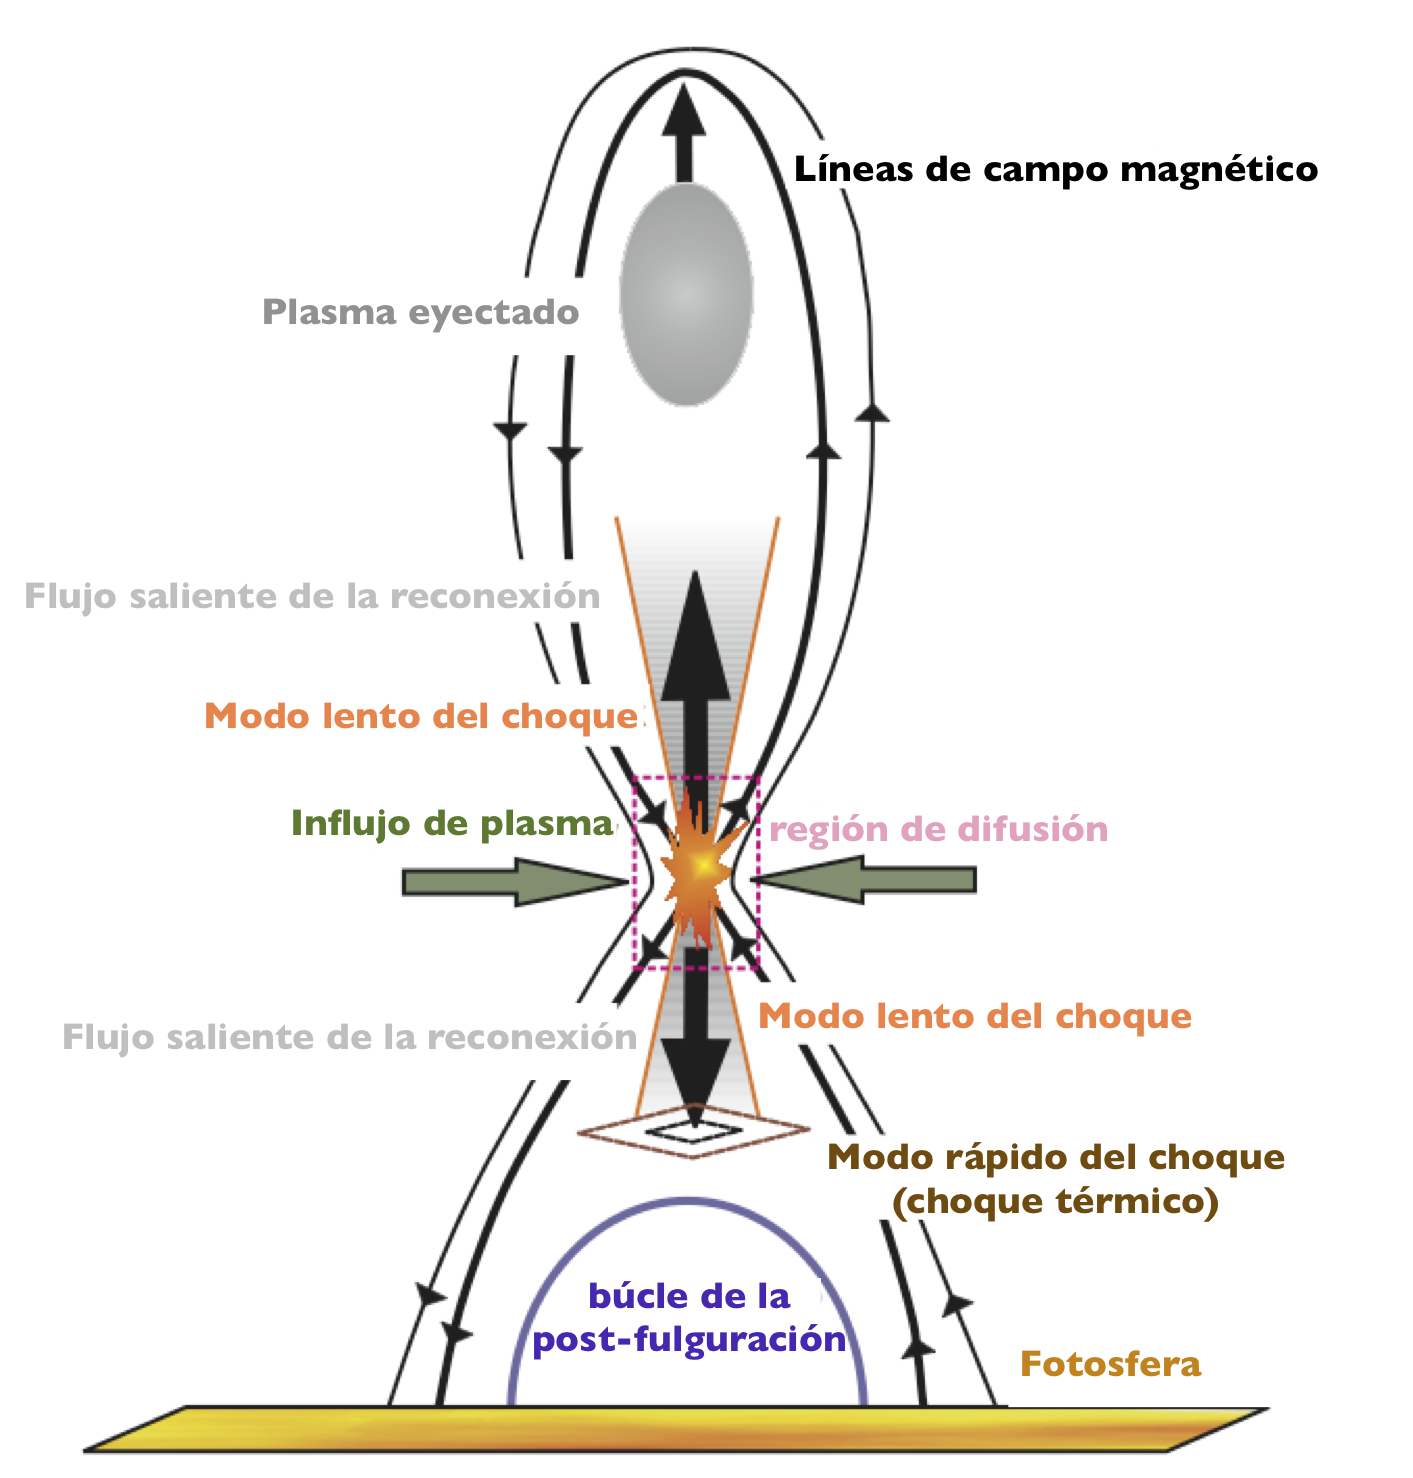
\includegraphics[width=0.65\textwidth]{reconexion.png}
\caption{Se representa esquem\'aticamente el proceso de reconexi\'on magn\'etica asociado a una fulguraci\'on solar. El evento ocurre en la regi\'on de difusi\'on de manera que el plasma local es catapultado hacia arriba y hacia abajo del v\'ertice de reconexi\'on en forma de jets de plasma.}
\label{reconexion}
\end{figure}

Una fulguraci\'on tiene su origen en un proceso de reconexi\'on magn\'etica. Cuando de la capa base de la fotosfera emergen l\'ineas de campo magn\'etico hacia la corona solar se posibilita la formaci\'on de una prominencia que, si tiene una configuraci\'on como la que se muestra en la figura \ref{reconexion}, genera las condiciones necesarias para que se presente un evento de reconexi\'on magn\'etica y, asociado a \'el, una fulguraci\'on solar. As\'i, en ese momento se establece una l\'amina de corriente que, si  excede un valor cr\'itico, provoca que la resistividad se incremente, debido a la excitaci\'on ondulatoria del plasma, originando de esta manera varios lugares de inestabilidad. En este caso la reconexi\'on magn\'etica puede ocurrir en la regi\'on donde la resistividad ha aumentado, i.e. la regi\'on de difusi\'on.

\subsection*{Clasificaci\'on de las fulguraciones}
\addcontentsline{toc}{subsection}{Clasificaci\'on de las fulguraciones}

Las fulguraciones se clasifican seg\'un la intensidad que se registra en rayos-X en un rango espectral que va de 1$\AA\,$a 8$\AA\,$ a trav\'es de los instrumentos de {\it GOES}\footnote{{\it GOES} es el acr\'onimo en ingl\'es de ``{\it Geostacionary Operational Environmental Satellite}'', ver http://www.swpc.noaa.gov/} \citep[]{fletcher2011}. Los valores t\'ipicos de potencia en una fulguraci\'on oscilan entre $10^{-8}$ W/m$^2$ y $10^{-3}$ W/m$^2$ de forma que es apenas natural pensar en una clasificaci\'on en escala logar\'itmica como la que se muestra en la figura \ref{goes}. Adicionalmente cada una de estas clases est\'a dividida en nueve subclases, i.e., la fulguraci\'on de clase X6 que se muestra en la figura \ref{goes}, o sea una intensidad de $6\times10^{-4}$ W/m$^2$, fue tres veces m\'as fuerte que la fulguraci\'on de clase X2 que se muestra en la misma figura, que a su vez fue cuatro veces m\'as fuerte que la fulguraci\'on de clase M5. Un resumen de esta clasificaci\'on se muestra en la tabla \ref{tabla_clas}


\begin{table}[htdp!]
\caption{Clasificaci\'on GOES de las fulguraciones solares}
\begin{center}
\begin{tabular}{|c|c|}\hline
Flujo [Wm$^{-2}$] & Clase GOES \\\hline
$10^{-8}$ & A1 \\
$10^{-7}$ & B1 \\
$10^{-6}$ & C1 \\
$10^{-5}$ & M1 \\
$10^{-4}$ & X1 \\
$10^{-3}$ & X10 \\\hline
\end{tabular}
\end{center}
\label{tabla_clas}
\end{table}

\subsection*{Inyecci\'on de part\'iculas energ\'eticas}
\addcontentsline{toc}{subsection}{Inyecci\'on de part\'iculas energ\'eticas}

Con ayuda de las observaciones llevadas a cabo por los diferentes telescopios espaciales durante las \'ultimas dos d\'ecadas \citep[]{aschwanden2004} se ha podido establecer que en el momento en que ocurre una explosi\'on solar asociada a una fulguraci\'on, una gran cantidad de part\'iculas cargadas el\'ectricamente se aceleran y son llevadas a niveles muy altos de energ\'ia (relativistas) en tan solo unos cuantos segundos, pero el mecanismo por medio del cual se desarrolla este proceso es a\'un tema de debate hoy d\'ia en la rama de la f\'isica solar. Los procesos de colisi\'on, ya sea v\'ia Coulomb o contra part\'iculas el\'ectricamente neutras, son mecanismos en los cuales en vez de existir una ganancia neta de energ\'ia por parte de las part\'iculas incidentes se presenta una p\'erdida. 

\begin{wrapfigure}[22]{r}{0.6\textwidth}
\centering
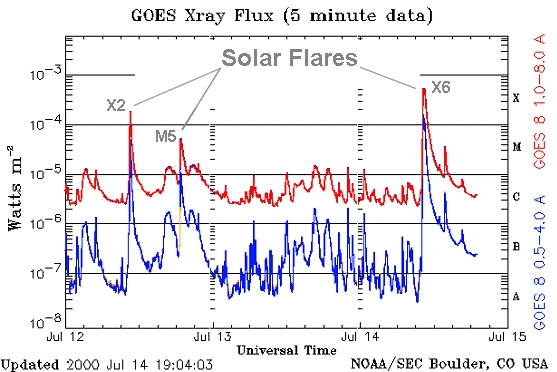
\includegraphics[width=0.58\textwidth]{goes.jpg}
\caption{El diagrama muestra la intensidad en rayos-X dada por {\it GOES} en un periodo de tiempo comprendido entre el 12 de Julio y el 15 de Julio del 2000. Durante este tiempo se observaron unas cuantas fulguraciones de diferentes tipos. Referencia: http://www.spaceweather.com/glossary/images/xray.gif }
\label{goes}
\end{wrapfigure}


Una forma natural de considerar la manera en la que se pueden acelerar estas part\'iculas y abastecerlas de la suficiente energ\'ia es suponiendo que se encuentran sometidas al efecto de un campo el\'ectrico particular. Recientemente muchos trabajos se han encaminado en esta direcci\'on \citep[]{HOLMAN1985,benz1987,ls1993,Tsuneta1998} teniendo alg\'un \'exito solo en el caso de poder reproducir par\'ametros estimados de las observaciones tales como las curvas de luz, los espectros y/o las densidades de part\'iculas. Es importante aclarar que la diferencia m\'as notoria entre estos modelos radica en la forma, lugar y momento en el que consideran la creaci\'on del campo, su topolog\'ia y la magnitud del mismo. Todos estos modelos de aceleraci\'on de part\'iculas est\'an cambiando continuamente a causa del  aumento constante en la calidad de las observaciones, y por ende, las resoluciones espacial y temporal de las mismas. Por ejemplo, hoy en d\'ia RHESSI es el sat\'elite que con una instrumentaci\'on apropiada ha permitido desarrollar investigaciones encaminadas a entender los procesos de aceleraci\'on de part\'iculas, por sus rangos din\'amico y espectral, resoluci\'on espectral y cadencia.\\

Como ya se ha mencionado, cuando se presenta un evento tipo {\it fulguraci\'on solar} un gran n\'umero de iones y electrones son acelerados y llevados a estados energ\'eticos relativistas \citep[]{2004emslie}. Estas part\'iculas se propagan a lo largo de las l\'ineas de campo magn\'etico y si contienen la cantidad de energ\'ia suficiente para alcanzar zonas m\'as densas de la atm\'osfera solar que se encuentran situadas m\'as abajo; estas pueden producir la emisi\'on de rayos X duros y gamma al colisionar con el plasma local \citep[]{Brown1971}. Entonces, durante las fulguraciones la radiaci\'on {\it no-t\'ermica} en rayos-X es producida principalmente v\'ia procesos de frenado {\it Bremsstrahlung} por las part\'iculas energ\'eticas que se propagan a trav\'es de la cromosfera densa. De aqu\'i que el espectro (de fotones) en rayos-X est\'a fuertemente relacionado con el espectro de las part\'iculas aceleradas en este evento. 

\subsection*{Una vista multi-frecuencia de las fulguraciones solares}
\addcontentsline{toc}{subsection}{Una vista multi-frecuencia de las fulguraciones solares}

El Sol luce completamente diferente dependiendo de la longitud de onda en la que se le observe. En la figura \ref{multi-frecuencia} se pueden ver las diferentes caras del Sol (para un mismo tiempo) cuando se observa en el visible (arriba a la izquierda), en H$\alpha$ (arriba a la derecha), en ultravioleta (abajo a la izquierda) y en rayos X (abajo a la derecha). 

La emisi\'on en rayos-X usualmente se origina en la corona, en las fulguraciones solares, o en regiones de la cromosfera alta cuando esta es calentada. En zonas de sol calmo la emisi\'on observada es una emisi\'on t\'ermica continua del plasma caliente y que se da gracias a las transiciones tipo {\it libre-libre} de los iones y electrones que se encuentran all\'i.  La figura \ref{corona-heating} ilustra la temperatura y densidad electr\'onica t\'ipica de la atm\'osfera en regiones de sol calmo \citep[]{benz2002}.\\

La emisi\'on en rayos-X obtenida del Sol se clasifica en rayos-X blandos y rayos-X duros.\\

{\it Rayos-X blandos}: ({\it SXR} por sus siglas en ingl\'es, {\it Soft X Rays}). Se considera que es emisi\'on t\'ermica producida por los iones y electrones energ\'eticos que conforman la atm\'osfera solar y la cual se caracteriza por la temperatura a la que se encuentre el plasma local. Las energ\'ias t\'ipicas de los fotones asociadas a este proceso oscilan en un rango de $\approx 0.1-15$ keV, es decir, en el rango de 0.8 a 124 $\AA$.\\


\begin{SCfigure}
\centering
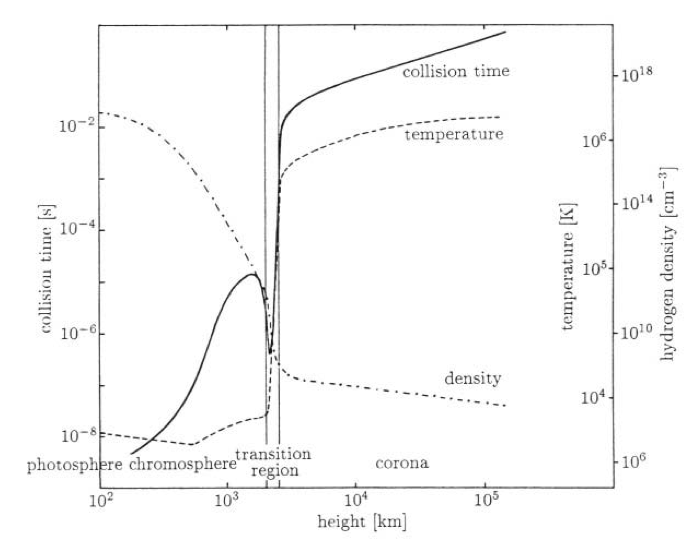
\includegraphics[width=0.48\textwidth]{corona-heating.png}
\caption{Curvas tomadas de \citep[]{benz2002} p\'agina 19. Aunque esta gr\'afica tiene bastante informaci\'on lo que nos interesa son las dos curvas punteadas correspondientes a la variaci\'on de la temperatura y de la densidad de hidr\'ogeno con respecto a la altura en la atm\'osfera solar. Estas curvas muestran una variaci\'on s\'ubita en la as\'i llamada {\it regi\'on de transici\'on} y su comportamiento es determinado suponiendo una regi\'on de sol calmo. La densidad decrece en ocho ordenes de magnitud y la temperatura crece en dos. Estos cambios abruptos a\'un hoy son temas que se consideran problemas abiertos de la f\'isica solar.}
\label{corona-heating}
\end{SCfigure}

{\it Rayos-X duros}: ({\it HXR} por sus siglas en ingl\'es: {\it Hard X Rays}) Es aquella emisi\'on de fotones con energ\'ias por encima de la energ\'ia que caracteriza los SXR, 300 keV (0.04 $\AA$), producidos por radiaci\'on de frenado ({\it Bremsstrahlung}) cuando el jet de part\'iculas aceleradas durante el evento de la fulguraci\'on colisiona con el plasma de la atm\'osfera local, aquello que se conoce en la literatura especializada como {\it thick} y {\it thin target}. Un an\'alisis detallado de las implicaciones f\'isicas asociadas a la emisi\'on en esta banda se encuentra en \citep[]{holman2011}.


\begin{figure}[ht!]
\centering
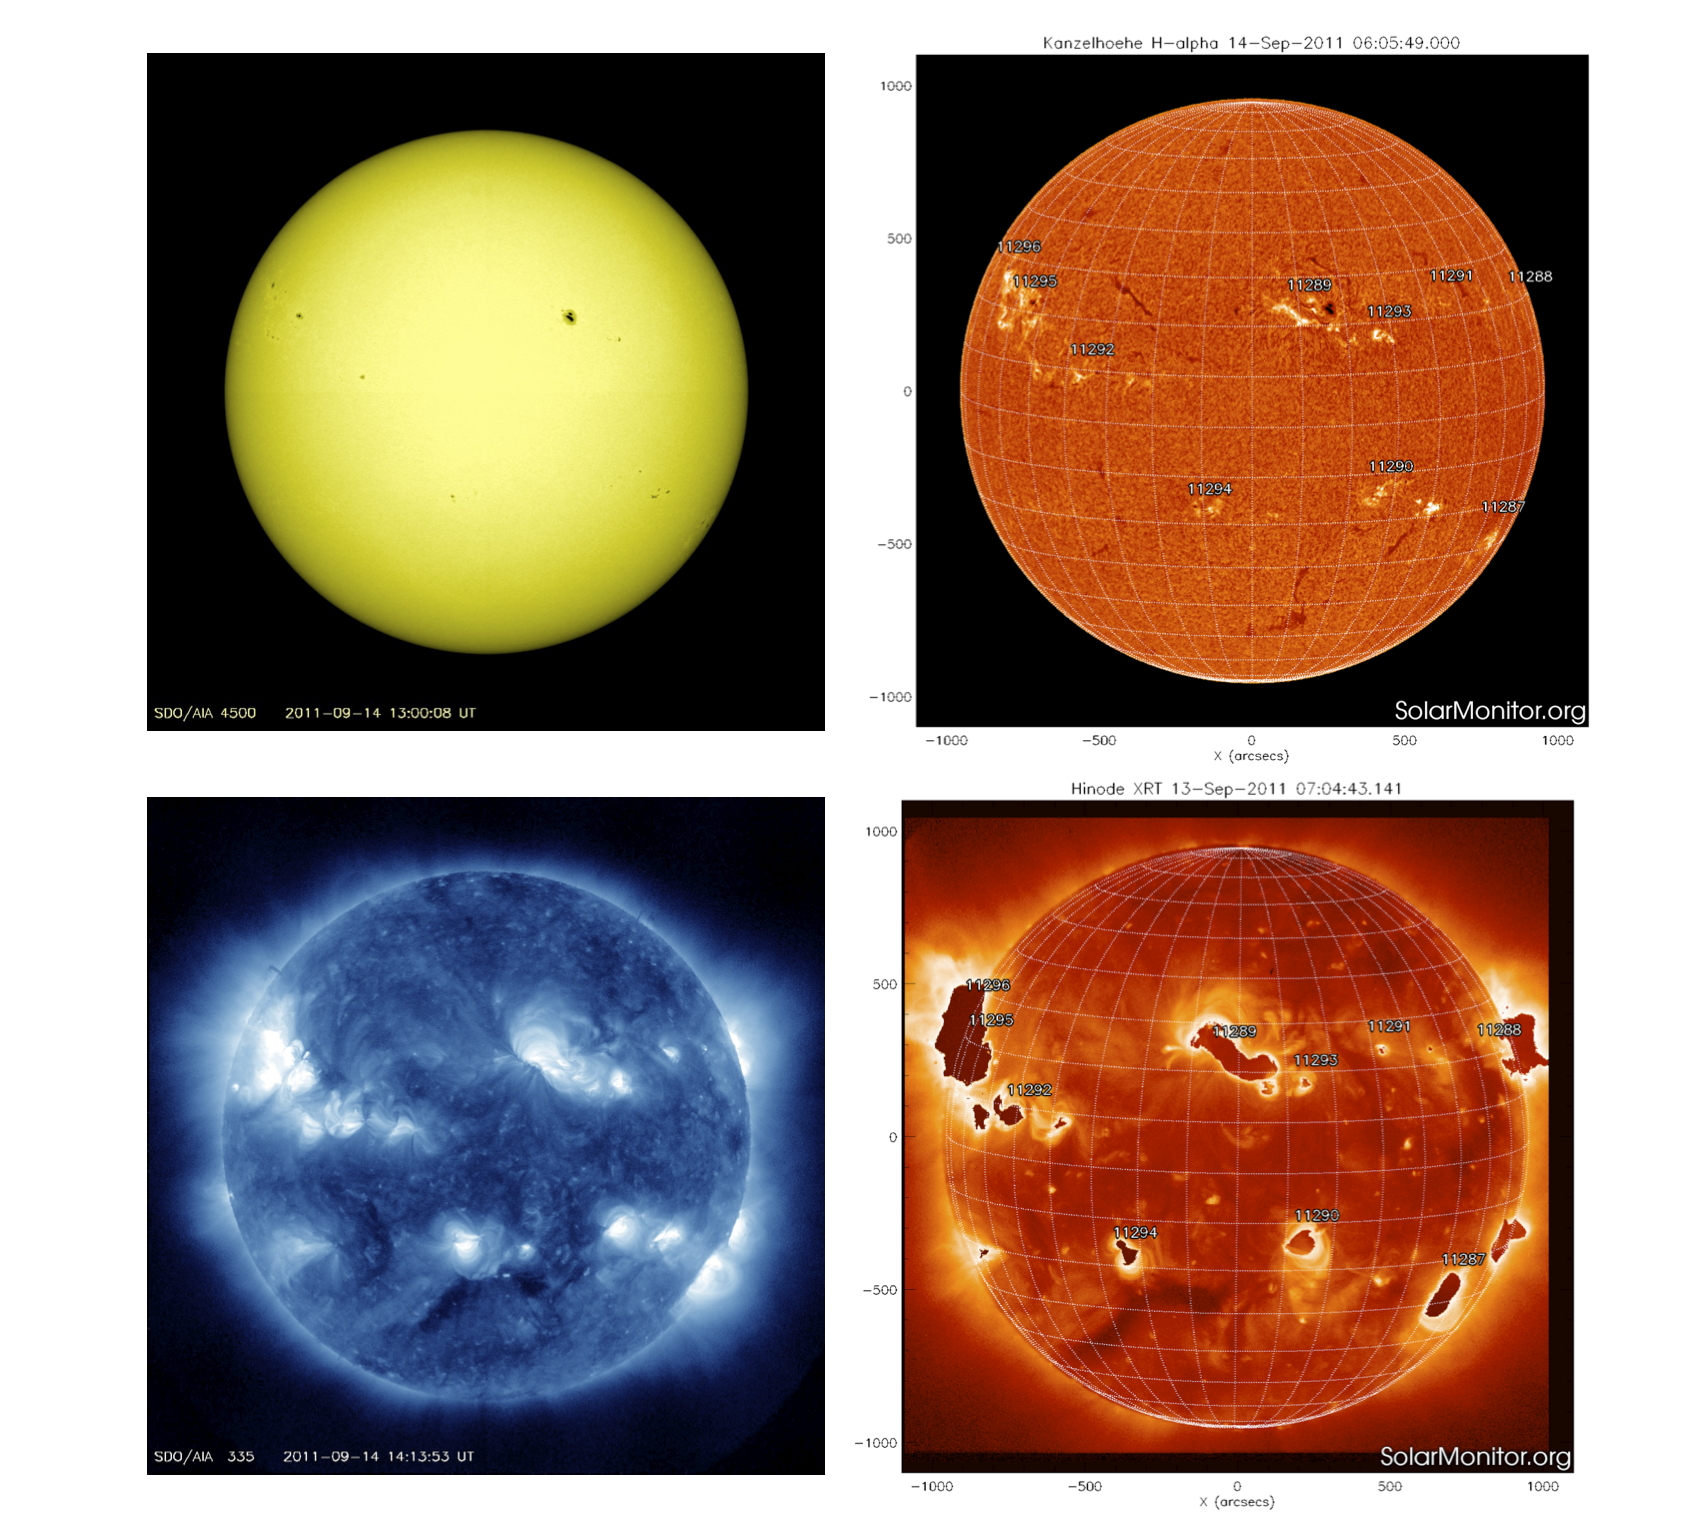
\includegraphics[width=0.91\textwidth]{multifrecuencia.png}
\caption{Visualizaci\'on del disco solar en diferentes bandas del espectro electromagn\'etico para el 14 de Septiembre de 2011. {\it Arriba a la izquierda:} Imagen del Sol en el continuo de luz blanca, mostrando 10 regiones activas, tomada por SDO/HMI (NASA) centrada en $4500\,\AA$. {\it Arriba a la derecha:} Imagen del Sol centrada en la l\'inea de H$\alpha$ ($6562,8\,\AA$) mostrando la estructura de la cromosfera tomada por el observatorio {\it Kanzelhoehe} de Austria. En esta imagen las prominencias se ven como filamentos oscuros sobre el disco solar. {\it Abajo a la izquierda:} Imagen en extremo ultravioleta tomada con un filtro centrado a $335\,\AA$ por SDO/AIA en donde se ilustra la regi\'on alta de transici\'on a una temperatura cercana a los 430.000 K. {\it Abajo a la derecha:} Imagen en rayos-X (centrado a $6\,\AA$) en donde se muestra la corona solar a una temperatura de unos 2 Millones de Kelvin tomada con el {\it Hinode} (Solar-B, JAXA/NASA/PPARC).}
\label{multi-frecuencia}
\end{figure}





